\section{Second Part (Non-Rigid structure from motion by factorization and assuming a low-rank trajectory model)}
\noindent In this section, we calculate the reconstruction with the low-rank trajectory method. This method is a little simpler because we already know in advance the matrix of base trajectories since we defined them with the value of k, we will show the structure in Equation \ref{eq:shape_trajectory}.
\begin{equation*}
	\theta=
	\begin{pmatrix}
		\theta_{1}^{1} &  \cdots & \theta_{k}^{1}\\		
		\vdots &  \ddots & \vdots \\
		\theta_{1}^{f} &  \cdots & \theta_{k}^{f}\\		
	\end{pmatrix}_{f\times k}
\end{equation*}
\begin{equation*}
	[a^{x}]=
	\begin{pmatrix}
		a_{11}^{x} &  \cdots & a_{1p}^{x}\\		
		\vdots &  \ddots & \vdots \\
		a_{k1}^{x} &  \cdots & a_{kp}^{x}\\		
	\end{pmatrix}_{k\times p}\text{ , }
	[a^{y}]=
	\begin{pmatrix}
		a_{11}^{y} &  \cdots & a_{1p}^{y}\\		
		\vdots &  \ddots & \vdots \\
		a_{k1}^{y} &  \cdots & a_{kp}^{y}\\		
	\end{pmatrix}_{k\times p}\text{ and }
	[a^{z}]=
	\begin{pmatrix}
		a_{11}^{z} &  \cdots & a_{1p}^{z}\\		
		\vdots &  \ddots & \vdots \\
		a_{k1}^{z} &  \cdots & a_{kp}^{z}\\		
	\end{pmatrix}_{k\times p}
\end{equation*}

\begin{equation}\label{eq:shape_trajectory}	
	\underbrace{\begin{pmatrix}
		x_{1}^{1} & x_{2}^{1} & \cdots & x_{p}^{1}\\
		y_{1}^{1} & y_{2}^{1} & \cdots & y_{p}^{1}\\
		z_{1}^{1} & z_{2}^{1} & \cdots & z_{p}^{1}\\
		\vdots & \vdots & \ddots & \vdots \\
		x_{1}^{f} & x_{2}^{f} & \cdots & x_{p}^{f}\\
		y_{1}^{f} & y_{2}^{f} & \cdots & y_{p}^{f}\\
		z_{1}^{f} & z_{2}^{f} & \cdots & z_{p}^{f}\\
	\end{pmatrix}}_{X}=
	\underbrace{\begin{pmatrix}
		\theta_{f\times k} & 0_{f\times k} & \cdots & 0_{f\times k} \\		
		0_{f\times k} &  \theta_{f\times k} & \vdots & 0_{f\times k}\\
		\vdots &  \vdots &\ddots & \vdots \\
		0_{f\times k} & 0_{f\times k} &  \cdots & \theta_{f\times k}		
	\end{pmatrix}}_{C}
	\underbrace{\begin{pmatrix}
				[a^{x}]_{k\times p} \\		
				[a^{y}]_{k\times p} \\
				[a^{z}]_{k\times p}				
		\end{pmatrix}}_{D}
\end{equation} 
\noindent Where $C$ is called trajectory bases and $D$ is called coefficients.\\

\noindent The low-rank trajectory method is optimized using the factorization method with SVD as shown in the lecture slide in Figure \ref{fig:slideT3}.\\

\begin{figure}[h]
	\centering
	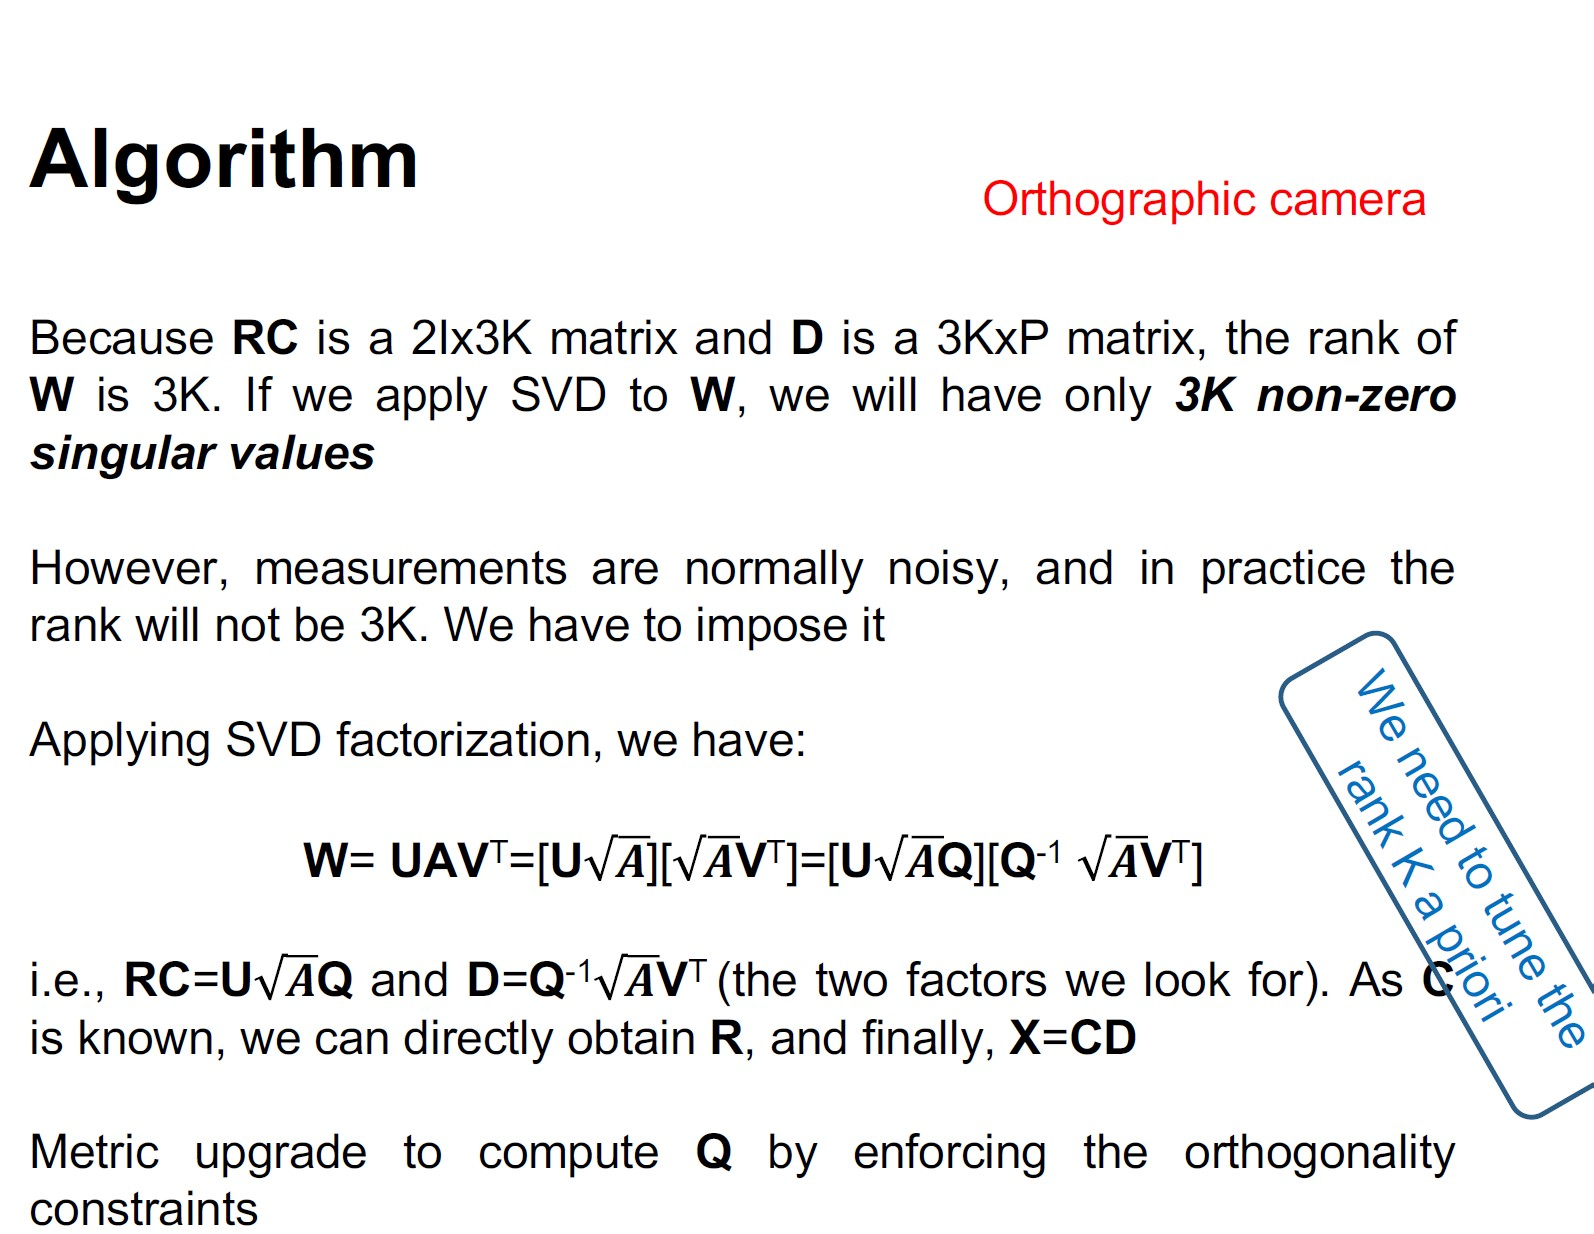
\includegraphics[width=0.7\textwidth]{T3/slide}
	\caption{Factoring slide}
	\label{fig:slideT3}
\end{figure}

\noindent As shown in Figure \ref{fig:slideT3}, in this case, the range of the matrix $W$ (measurement matrix) is $3k$ since $RC$ is of dimension $2I\times 3k$ and $D$ is of dimension $3k\times p$. Therefore, we must calculate $Q$ by enforcing the orthogonality constraints for $RC$ ($RCxRC'=I_{2Ix2I}$) and since $C$ is already known, we can calculate $X$ in the form $X=CD$.\\
\subsection{Code:}
\noindent Now we will show how to update $Q$ to find the shape matrix $X$.
\begin{lstlisting}[style=Matlab-editor, numbers=left]
	[U,D,V]=svd(W,0);
	RHat=U(:,1:3*K)*sqrt(D(1:3*K,1:3*K));
	Xhat=sqrt(D(1:3*K,1:3*K))*V(:,1:3*K)';    
	
	% Metric Upgrade step
	[Q] = metricUpgrade(RHat);
	Rsh = RHat*Q;
	% Computing final motion and shape
	R = recoverR(Rsh);
	C = DCT_basis(n_frames,K);
	G = R*C;
	D = inv(G'*G)*G'*W;
	X=C*D;
\end{lstlisting}
\noindent In the line 1, we compute the SVD by $W$ (measurement matrix)).\\
\noindent In the line 2 and 3, since we know the rank of the matrix is $3k$, then we restrict the dimensions of the matrices $U$, $D$, and $V$ as follows:
\begin{itemize}
	\item For $U$, we take only its first $3k$ columns.
	\item For $D$, we take only its first $3k$ rows and first 3 columns.
	\item For $V$ we take only the last $3k$ columns
\end{itemize}
\noindent And with these new restrictions for $U$, $D$ and $V$, we calculate the initials matrix $RC=U\sqrt{D}$ and $D=\sqrt{D}V'$.\\
\noindent In the line 6, We update Q by using the orthogonality conditions for the matrix $RHat*q$($RHat=$initial RC)
\begin{lstlisting}[style=Matlab-editor, numbers=left]
function [Q] = metricUpgrade(LambdaHat,q0)

k = size(LambdaHat,2)/3;
F = size(LambdaHat,1)/2;

if(~exist('q0'))
q0 = zeros(3*k,3);
q0(0*k+1,1) = 1;
q0(1*k+1,2) = 1;
q0(2*k+1,3) = 1;
end
options = optimset('Diagnostics','off','MaxFunEval',100000,'MaxIter',2000,'TolFun',1e-10,'TolX',1e-10);
[q, fval] = fminunc(@evalQ,q0,options,LambdaHat); 

Q = reshape(q,3*k,3);
\end{lstlisting}
as we can see inside the function $metricUpgrade(LambdaHat,q0)$ on line 13\\.
\noindent In the line 10, we compute the trajectory bases.\\
\noindent In the line 12, we calculate $D$ from $RC$, solving the equation $\Vert W-RCD\Vert =0$.\\
\noindent In the line 13, finally we calculate the shape matrix $X=CD$.\\
\subsection{Examples:}